\documentclass[12pt,a4paper]{article}
\usepackage[margin=1in]{geometry}
\usepackage{amsmath, amssymb, graphicx, hyperref, caption, booktabs, float, subcaption}

% Title Page
\title{PFITZER PROJECT}
\author{Pierre Jourdin \\ Aymeric Conti \\ Hadrien Crassous}

\begin{document}

\maketitle

\section*{Introduction}

La structure de base de notre modélisation gurobi est la suivante : on a nombre\_SR x nombre\_briques variables booléennes, chacune indiquant si le SR correspondant s'occupe de la brique correspondante (True) ou non (False).\\
Les fonctions suivantes sont définies en fonction de ces variables ainsi que des paramètres du problème :
\begin{itemize}
    \item compute\_distance
    \item compute\_workload
    \item compute\_disruption
\end{itemize}
Sauf indication contraire, la workload est traitée comme une contrainte : elle doit se situer dans un intervalle fixe (par exemple [0.8,1.2]).\\
Les changements de structure spécifiques aux différents problèmes sont détaillés au cours du rapport.

\section*{Step 1 : Briques Centrales Fixes}

\subsection*{Mono-objectif}

Les deux résolutions se font facilement avec la structure expliquée en Introduction, les résultats obtenus sont :
\begin{itemize}
    \item \textbf{Best disruption : 0.3391}
    \item \textbf{Best distance : 309.24}
\end{itemize}

\subsection*{Bi-objectif}
On implémente le schéma epsilon-constraint en optimisant la distance et en "fixant" la disruption.

résultats :

\begin{figure}[H]
    \centering
    \begin{subfigure}{0.32\textwidth}
        \centering
        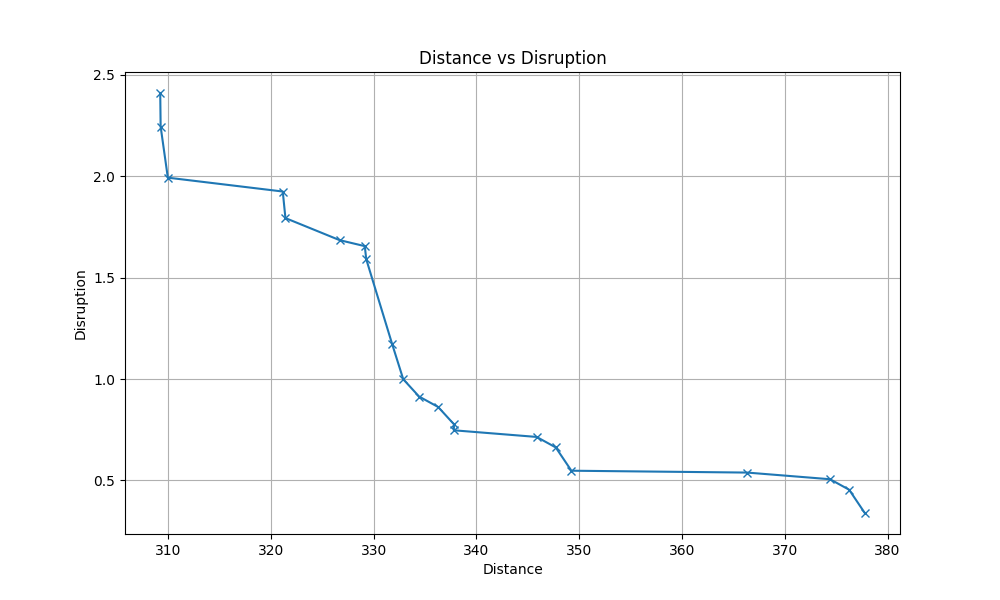
\includegraphics[width=\textwidth]{figures/solve1-0.8.png}
        \caption{0.8 - 1.2}
        \label{fig:solve1}
    \end{subfigure}
    \hfill
    \begin{subfigure}{0.32\textwidth}
        \centering
        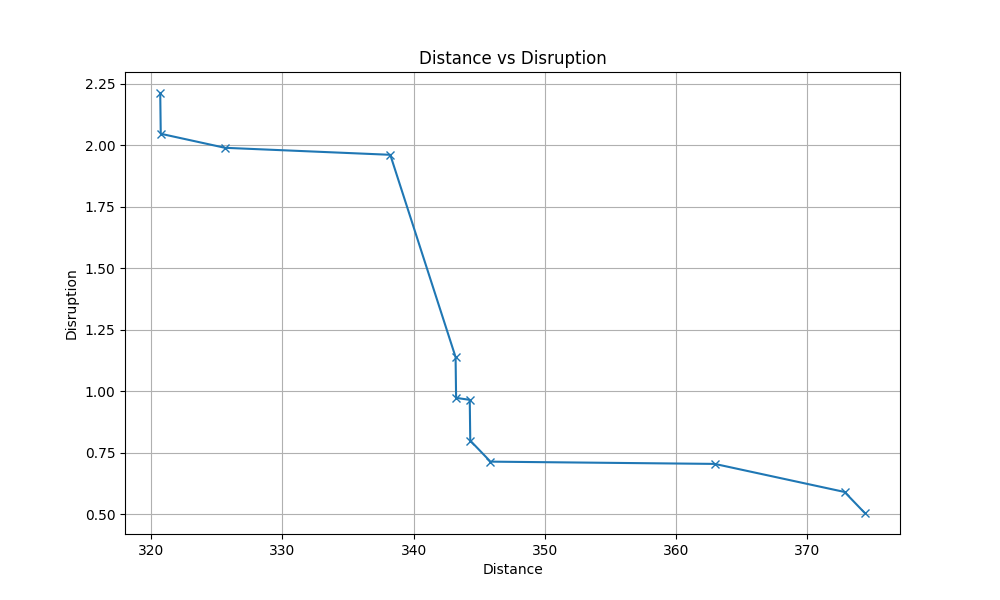
\includegraphics[width=\textwidth]{figures/solve1-0.85.png}
        \caption{0.85 - 1.15}
        \label{fig:solve2}
    \end{subfigure}
    \hfill
    \begin{subfigure}{0.32\textwidth}
        \centering
        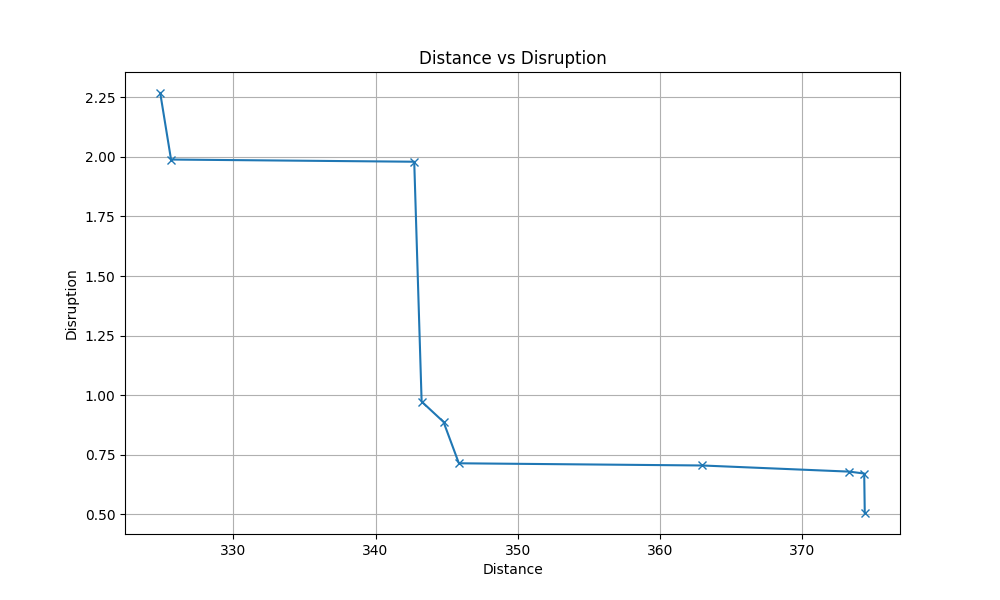
\includegraphics[width=\textwidth]{figures/solve1-0.9.png}
        \caption{0.9 - 1.1}
        \label{fig:solve3}
    \end{subfigure}
    \caption{Results for the bi-objective optimization.}
    \label{fig:all_solves}
\end{figure}

\subsection*{Instance plus grosse}

\begin{figure}[H]
    \centering
    \begin{subfigure}{0.32\textwidth}
        \centering
        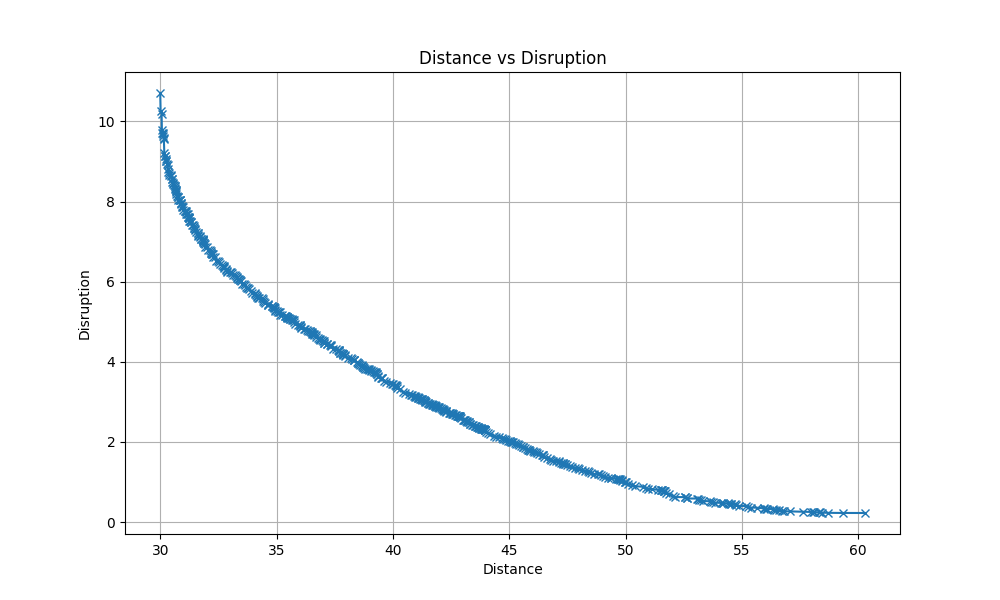
\includegraphics[width=\textwidth]{figures/solve1-100-0.8.png}
        \caption{0.8 - 1.2}
        \label{fig:solve1}
    \end{subfigure}
    \hfill
    \begin{subfigure}{0.32\textwidth}
        \centering
        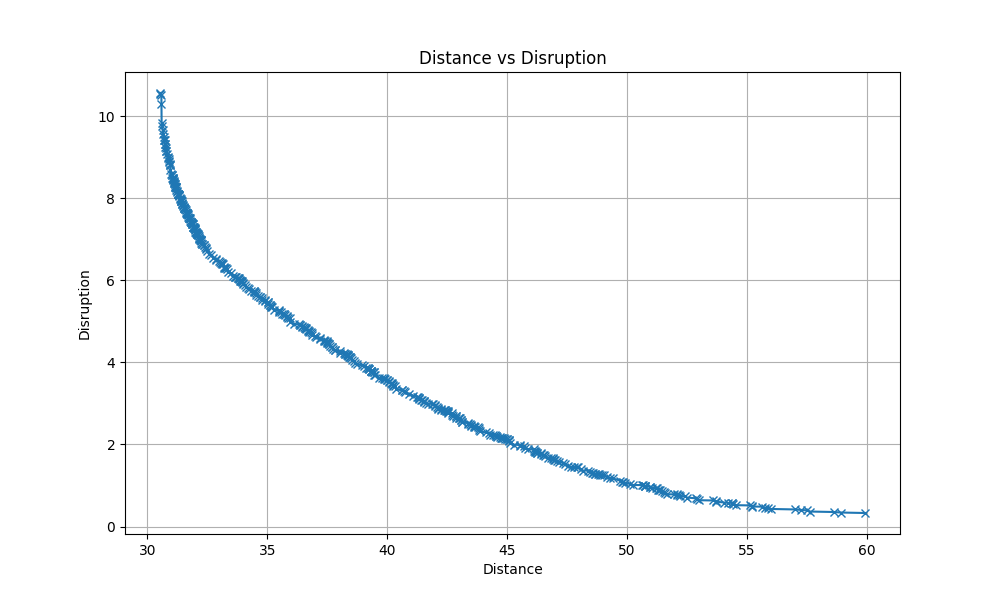
\includegraphics[width=\textwidth]{figures/solve1-100-0.85.png}
        \caption{0.85 - 1.15}
        \label{fig:solve2}
    \end{subfigure}
    \hfill
    \begin{subfigure}{0.32\textwidth}
        \centering
        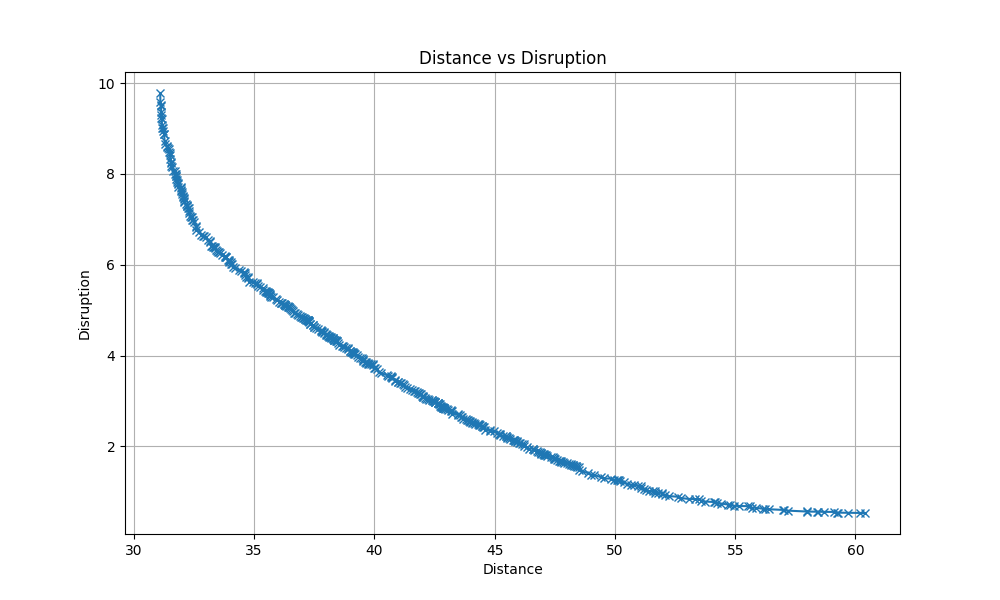
\includegraphics[width=\textwidth]{figures/solve1-100-0.9.png}
        \caption{0.9 - 1.1}
        \label{fig:solve3}
    \end{subfigure}
    \caption{Results for the bi-objective optimization with 100 SR and 100 bricks.}
    \label{fig:all_solves}
\end{figure}

\section*{Step 2 : Extensions du Modèle}

\subsection*{Assignation partielle des briques}
Ici, on fait l'hypothèse que, si un SR est assigné partiellement à une brique, il a une workload partielle de la workload totale de la brique (au prorata); Idem pour les disruptions. En revanche, le SR doit tout de même faire l'entièreté du déplacement vers la brique si il a été assigné à une partie non nulle de la brique.
\\
Modification du modèle : les nombre\_SR x nombre\_briques variables ne sont plus booléennes mais entre 0 et 1, et doivent vérifier que la somme pour chaque brique vaut 1.
On a aussi ajouté 2 x nombre\_SR x nombre\_briques variables booléennes pour implémenter le modèle.
\\

\begin{figure}[H]
    \centering
    \begin{subfigure}{0.32\textwidth}
        \centering
        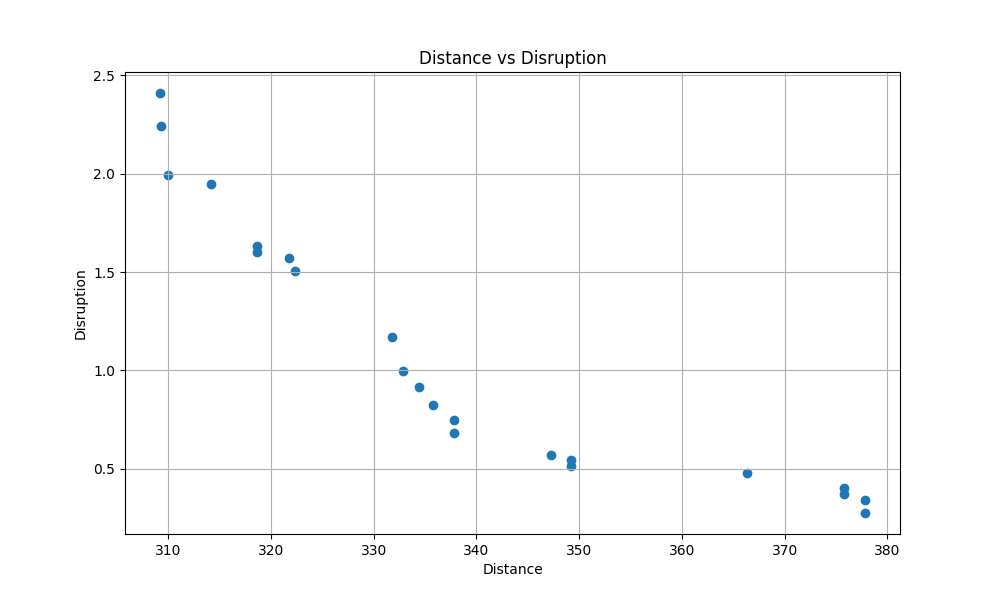
\includegraphics[width=\textwidth]{figures/solve2-0.8.png}
        \caption{0.8 - 1.2}
        \label{fig:solve1}
    \end{subfigure}
    \hfill
    \begin{subfigure}{0.32\textwidth}
        \centering
        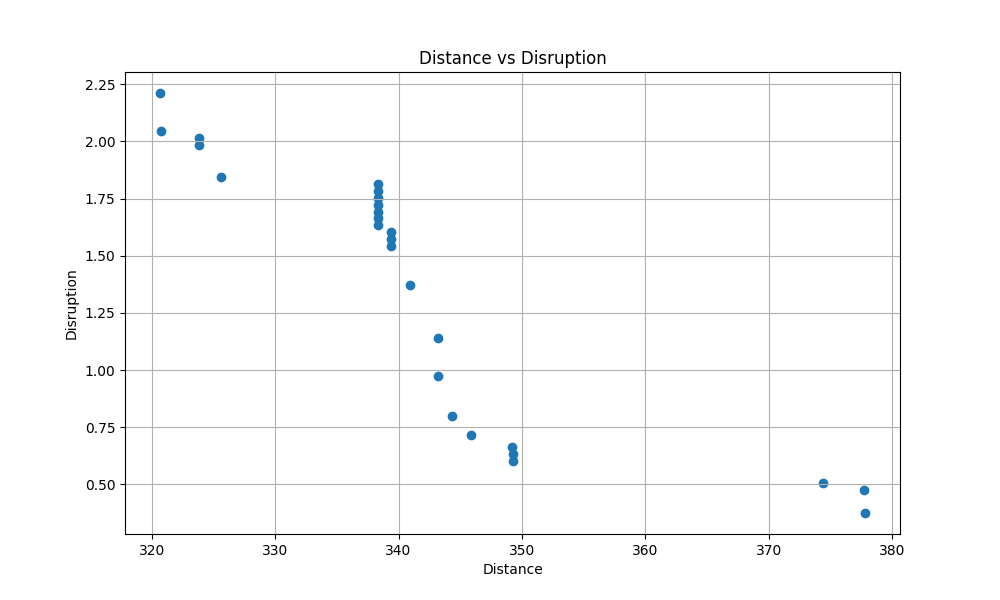
\includegraphics[width=\textwidth]{figures/solve2-0.85.png}
        \caption{0.85 - 1.15}
        \label{fig:solve2}
    \end{subfigure}
    \hfill
    \begin{subfigure}{0.32\textwidth}
        \centering
        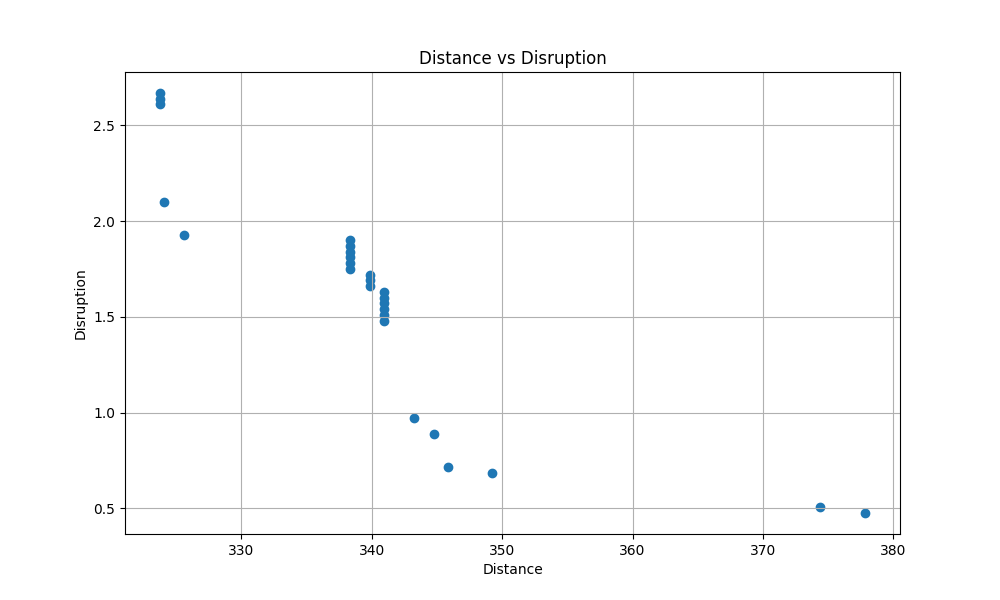
\includegraphics[width=\textwidth]{figures/solve2-0.9.png}
        \caption{0.9 - 1.1}
        \label{fig:solve3}
    \end{subfigure}
    \caption{Results for the bi-objective optimization with partial assignment.}
    \label{fig:all_solves}
\end{figure}

\subsection*{Ajout d'un nouveau SR}

On doit ajouter un cinquième SR pour combler le 25\% de travail en plus. On peut choisir l'emplacement de son bureau.\\
Pour faire cela, on ajoute nombre\_briques variables binaires, dont une unique vaut 1 encodant la position du nouveau bureau. De plus, on utilise QuadExpr() au lieu de LinExpr() pour pouvoir multiplier deux variables entre elles (le temps de calcul reste raisonnable).

\begin{figure}[H]
    \centering
    \begin{subfigure}{0.32\textwidth}
        \centering
        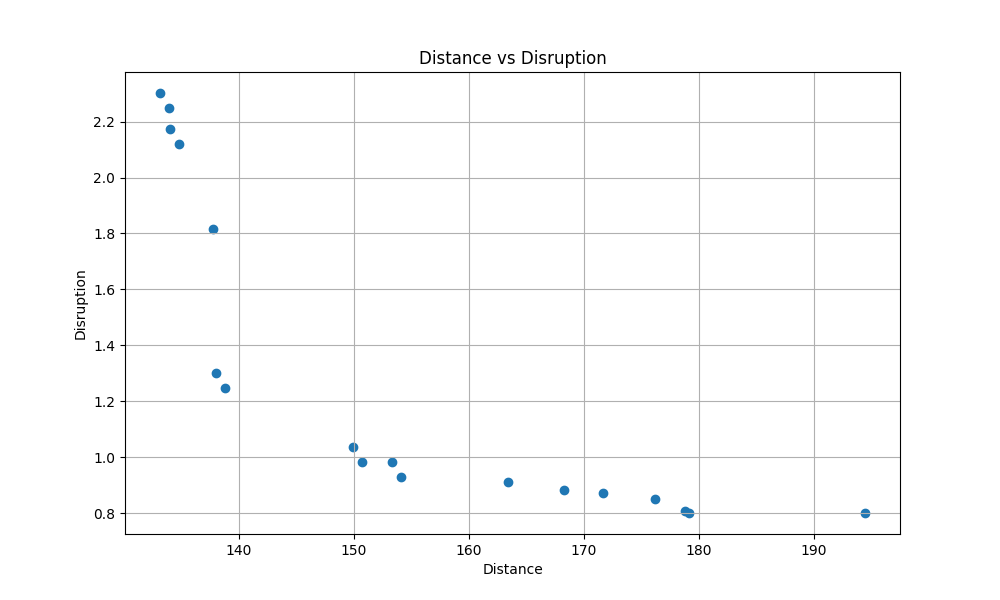
\includegraphics[width=\textwidth]{figures/solve3-0.8.png}
        \caption{0.8 - 1.2}
        \label{fig:solve1}
    \end{subfigure}
    \hfill
    \begin{subfigure}{0.32\textwidth}
        \centering
        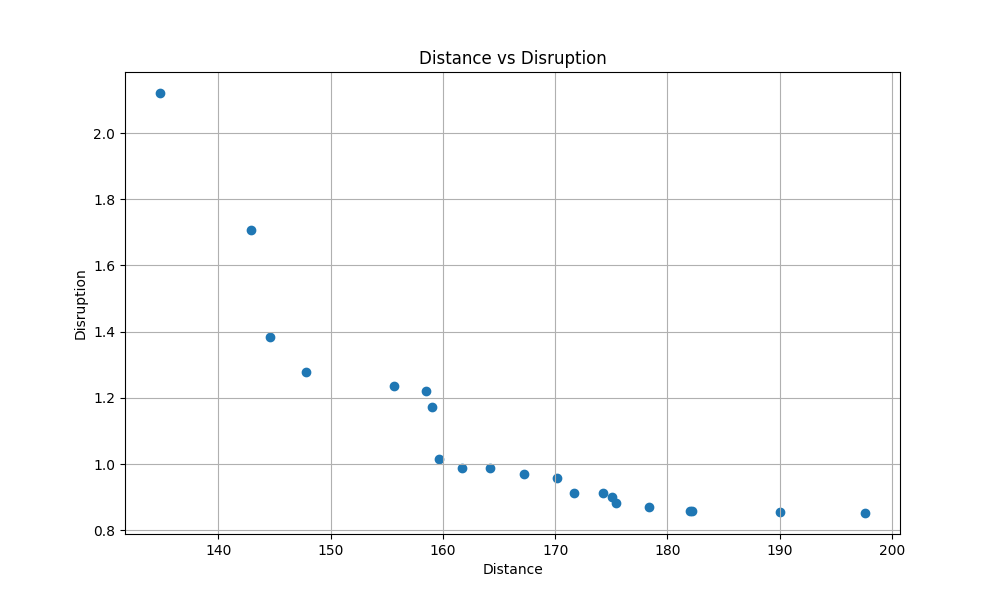
\includegraphics[width=\textwidth]{figures/solve3-0.85.png}
        \caption{0.85 - 1.15}
        \label{fig:solve2}
    \end{subfigure}
    \hfill
    \begin{subfigure}{0.32\textwidth}
        \centering
        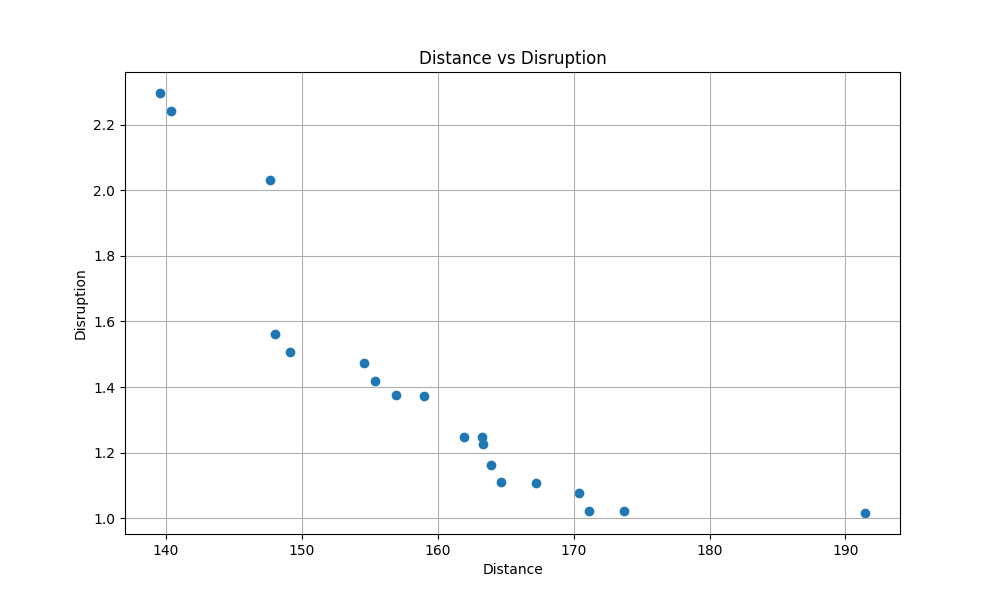
\includegraphics[width=\textwidth]{figures/solve3-0.9.png}
        \caption{0.9 - 1.1}
        \label{fig:solve3}
    \end{subfigure}
    \caption{Results for the bi-objective optimization with a new SR.}
    \label{fig:all_solves}
\end{figure}

\section*{Step 3 : Modification des Briques Centrales}

\subsection*{Bi-objectif avec positions des bureaux variables}
Les deux objectifs sont : distance et workload. On oublie la disruption dans cette section. Pour le workload, on le quantifie par l'écart au workload idéal : 1. On veut minimiser cet écart.\\
Ici, on utilise comme variables 2 tables de taille nombre\_SR x nombre\_briques chacune : une pour stocker les assignations des SR et l'autre pour stocker la position des bureaux. On utilise aussi QuadExpr() pour pouvoir multiplier les variables. (Il aurait aussi été possible d'utiliser LinExpr(), et d'avoir des variables correspondant à chacun des produits de deux variables dont on a besoin dans le calculs, mais on a préféré utiliser QuadExpr()).

\begin{figure}[H]
    \centering
    \begin{subfigure}{0.32\textwidth}
        \centering
        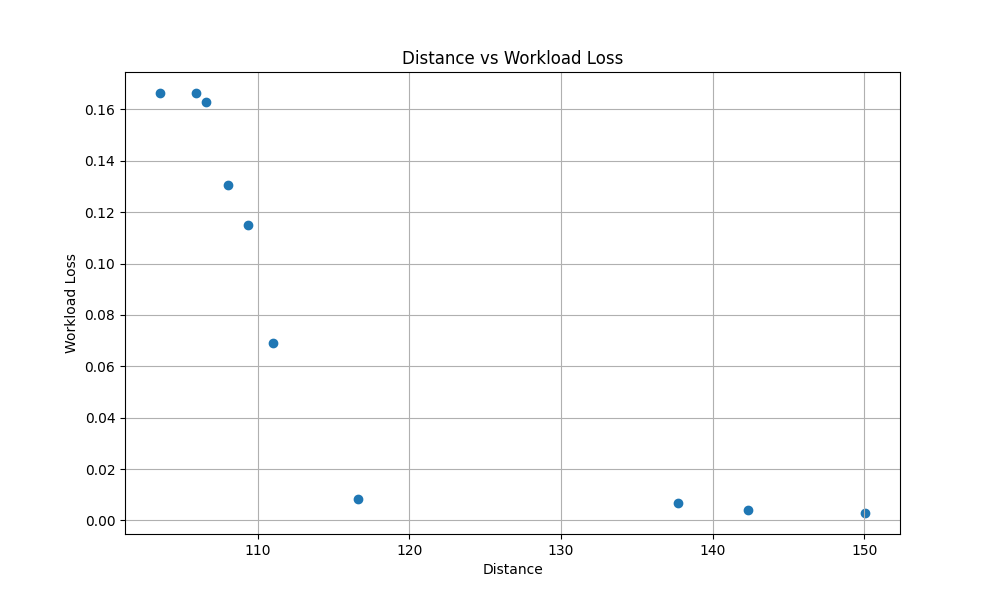
\includegraphics[width=\textwidth]{figures/solve4-0.8.png}
        \caption{0.8 - 1.2}
        \label{fig:solve1}
    \end{subfigure}
    \hfill
    \begin{subfigure}{0.32\textwidth}
        \centering
        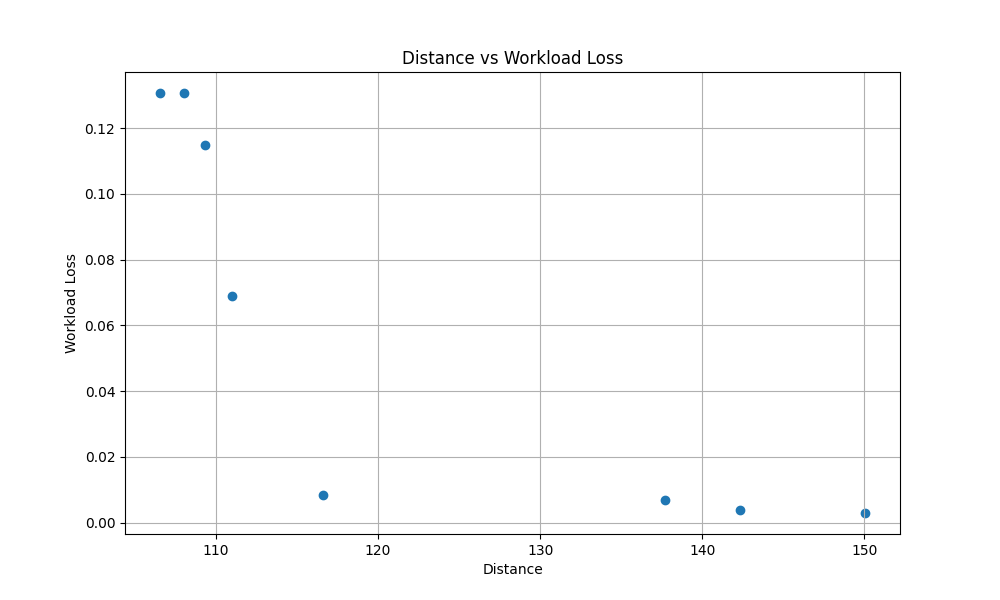
\includegraphics[width=\textwidth]{figures/solve4-0.85.png}
        \caption{0.85 - 1.15}
        \label{fig:solve2}
    \end{subfigure}
    \hfill
    \begin{subfigure}{0.32\textwidth}
        \centering
        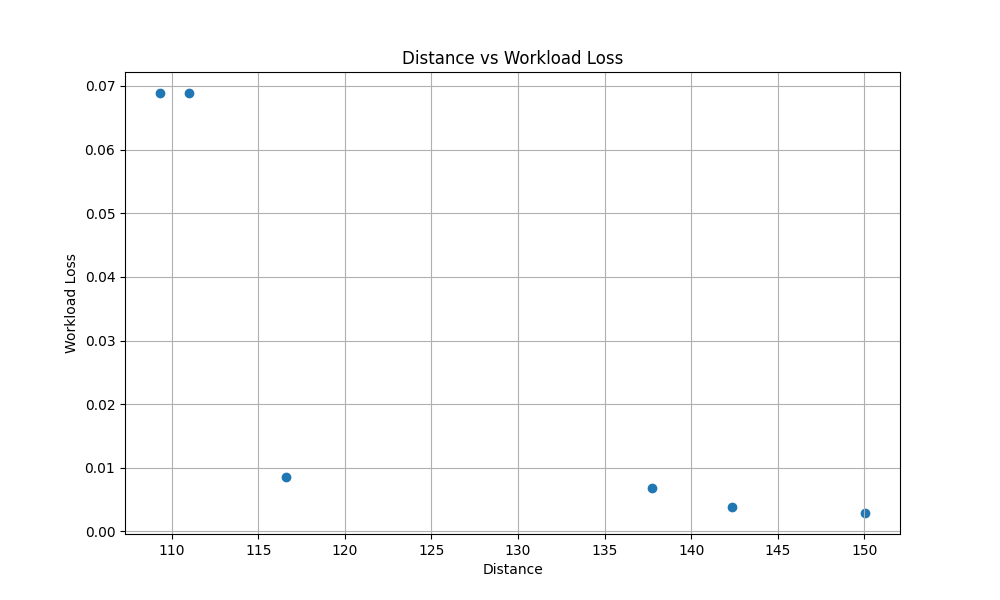
\includegraphics[width=\textwidth]{figures/solve4-0.9.png}
        \caption{0.9 - 1.1}
        \label{fig:solve3}
    \end{subfigure}
    \caption{Results for the bi-objective optimization with variable positions of the offices.}
    \label{fig:all_solves}
\end{figure}

\subsection*{Tri-objectif}
On utilise les 3 objectifs : distance, workload et disruption (nouvelle définition). On utilise un schéma epsilon-constraint double : On minimise la distance et on fixe des deux autres successivement. Voir le code pour les détails.

\begin{figure}[H]
    \centering
    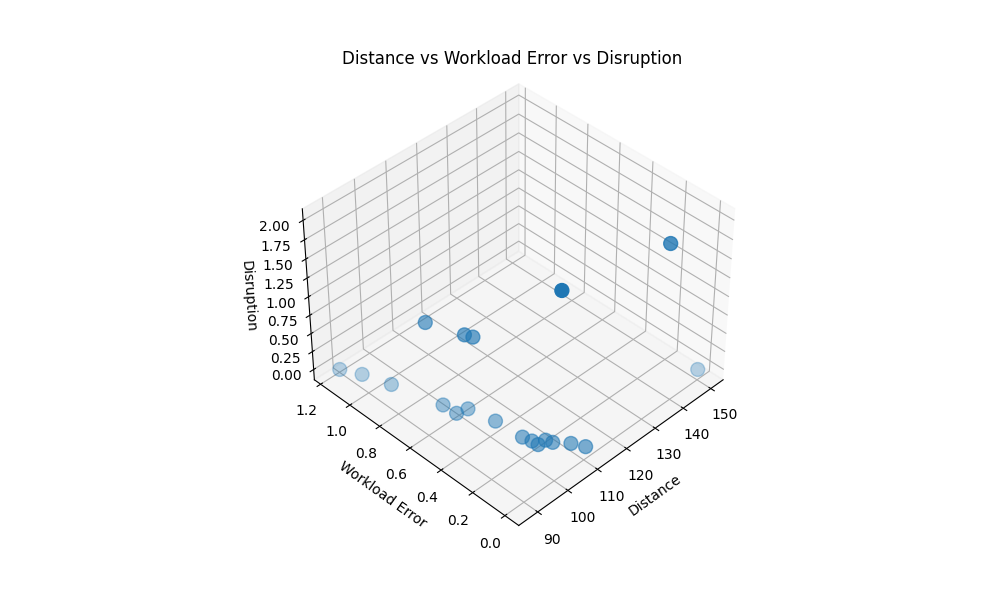
\includegraphics[width=0.8\textwidth]{figures/solve5.png}
    \caption{Results for the tri-objective optimization.}
    \label{fig:solve2}
\end{figure}

\section*{Step 4 : Sélection des Solutions}


\section*{Conclusion}

\end{document}